\documentclass[11pt]{article}

\usepackage[margin=0.82in,headheight=15pt]{geometry}
\usepackage{fontspec}
\usepackage{unicode-math}
\setmainfont{DejaVu Serif}
\setsansfont{DejaVu Sans}
\setmonofont[Scale=0.83]{DejaVu Sans Mono}
\setmathfont{DejaVu Math TeX Gyre}
\usepackage{microtype}
\usepackage{xcolor}
\usepackage{booktabs,tabularx,array,longtable,multirow}
\usepackage{enumitem}
\usepackage{fancyhdr}
\usepackage{titlesec}
\usepackage{tocloft}
\usepackage[most]{tcolorbox}
\usepackage{tikz}
\usetikzlibrary{arrows.meta,positioning,fit,backgrounds,calc,shapes.geometric,matrix}
\usepackage{listings}
\usepackage{hyperref}

\definecolor{navy}{HTML}{17324D}
\definecolor{blue}{HTML}{276FBF}
\definecolor{cyan}{HTML}{2A9D8F}
\definecolor{gold}{HTML}{E9A23B}
\definecolor{red}{HTML}{C94C4C}
\definecolor{ink}{HTML}{202A35}
\definecolor{muted}{HTML}{627282}
\definecolor{paper}{HTML}{F7F9FC}
\definecolor{line}{HTML}{D8E1EA}
\definecolor{codebg}{HTML}{F2F5F8}

\hypersetup{colorlinks=true,linkcolor=blue,urlcolor=blue,pdftitle={Reading Numbers.lean},pdfauthor={William Sollers}}
\pagestyle{fancy}
\fancyhf{}
\lhead{\small\sffamily Reading \texttt{Numbers.lean}}
\rhead{\small\sffamily Adventures in Mathematics}
\cfoot{\small\sffamily\thepage}
\renewcommand{\headrulewidth}{0.4pt}
\titleformat{\section}{\Large\bfseries\sffamily\color{navy}}{\thesection}{0.55em}{}
\titleformat{\subsection}{\large\bfseries\sffamily\color{blue}}{\thesubsection}{0.55em}{}
\titleformat{\subsubsection}{\normalsize\bfseries\sffamily\color{ink}}{\thesubsubsection}{0.55em}{}
\setlist{nosep,leftmargin=1.5em}
\setlength{\parindent}{0pt}
\setlength{\parskip}{5pt plus 1pt}
\emergencystretch=1em
\setlength{\cftsecnumwidth}{2.4em}
\setlength{\cftsubsecnumwidth}{3.2em}

\lstdefinelanguage{Lean}{
  morekeywords={class,structure,where,extends,instance,theorem,def,namespace,end,universe,Type,Prop,forall,fun,by,exact,rfl,variable,if,then,else},
  sensitive=true,
  morecomment=[l]{--},
  morecomment=[s]{/-}{-/},
  morestring=[b]"
}
\lstset{
  language=Lean,
  basicstyle=\ttfamily\small,
  keywordstyle=\color{blue}\bfseries,
  commentstyle=\color{muted}\itshape,
  stringstyle=\color{cyan!70!black},
  backgroundcolor=\color{codebg},
  frame=single,
  rulecolor=\color{line},
  framesep=5pt,
  xleftmargin=2pt,
  xrightmargin=2pt,
  breaklines=true,
  columns=fullflexible,
  keepspaces=true,
  showstringspaces=false,
  literate=
    {∀}{{$\forall$}}1 {→}{{$\to$}}1 {≤}{{$\le$}}1 {≥}{{$\ge$}}1
    {≠}{{$\ne$}}1 {∧}{{$\land$}}1 {∨}{{$\lor$}}1 {↔}{{$\leftrightarrow$}}1
    {∃}{{$\exists$}}1 {⁻¹}{{$^{-1}$}}1 {⟨}{{$\langle$}}1 {⟩}{{$\rangle$}}1
    {·}{{$\cdot$}}1 {:=}{{$:=$}}2
}

\newtcolorbox{bigidea}[1][]{enhanced,breakable,colback=blue!4,colframe=blue!65!black,
  boxrule=0.7pt,arc=2pt,left=7pt,right=7pt,top=6pt,bottom=6pt,
  fonttitle=\bfseries\sffamily,title={Big idea},#1}
\newtcolorbox{mental}[1][]{enhanced,breakable,colback=cyan!5,colframe=cyan!70!black,
  boxrule=0.7pt,arc=2pt,left=7pt,right=7pt,top=6pt,bottom=6pt,
  fonttitle=\bfseries\sffamily,title={Mental model},#1}
\newtcolorbox{warningbox}[1][]{enhanced,breakable,colback=gold!8,colframe=gold!80!black,
  boxrule=0.7pt,arc=2pt,left=7pt,right=7pt,top=6pt,bottom=6pt,
  fonttitle=\bfseries\sffamily,title={Watch this},#1}
\newtcolorbox{tracebox}[1][]{enhanced,breakable,colback=paper,colframe=navy!60,
  boxrule=0.7pt,arc=2pt,left=7pt,right=7pt,top=6pt,bottom=6pt,
  fonttitle=\bfseries\sffamily,title={Elaboration trace},#1}
\newcommand{\code}[1]{\texttt{\detokenize{#1}}}
\newcommand{\Lean}{Lean~4}

\tikzset{
  box/.style={draw=line,very thick,rounded corners=2pt,fill=white,align=center,
    minimum height=8mm,inner sep=5pt,font=\small\sffamily},
  data/.style={box,draw=blue!65,fill=blue!5},
  law/.style={box,draw=cyan!70!black,fill=cyan!5},
  bundle/.style={box,draw=navy,fill=navy!5,font=\small\bfseries\sffamily},
  generated/.style={box,draw=gold!80!black,fill=gold!8},
  arr/.style={-{Latex[length=2.2mm]},thick,draw=muted},
  infer/.style={-{Latex[length=2.2mm]},thick,dashed,draw=red!80!black},
}

\begin{document}

\begin{titlepage}
\begin{tikzpicture}[remember picture,overlay]
  \fill[navy] (current page.north west) rectangle ([yshift=-5.4cm]current page.north east);
  \fill[blue] ([yshift=-5.4cm]current page.north west) rectangle ([yshift=-5.55cm]current page.north east);
  \node[anchor=north west,text=white,font=\sffamily\bfseries\fontsize{28}{32}\selectfont,
    text width=15cm] at ([xshift=1.4cm,yshift=-1.45cm]current page.north west)
    {Reading \texttt{Numbers.lean}};
  \node[anchor=north west,text=blue!20,font=\sffamily\fontsize{15}{19}\selectfont,
    text width=14.5cm] at ([xshift=1.4cm,yshift=-3.1cm]current page.north west)
    {A visual guide to Lean syntax, mixins, structures, construction, and instance inference};
\end{tikzpicture}

\vspace*{5.7cm}
\begin{center}
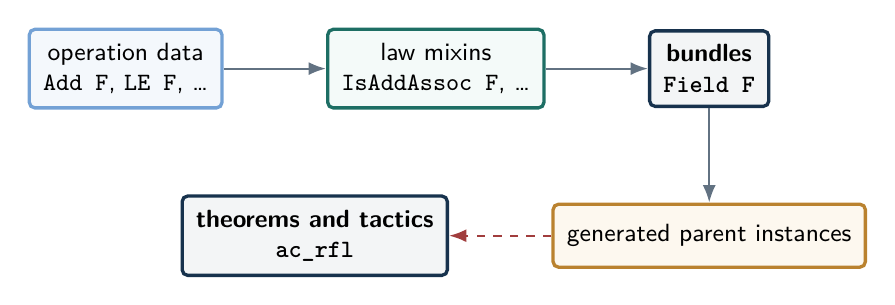
\begin{tikzpicture}[node distance=12mm and 13mm]
  \node[data] (ops) {operation data\\\code{Add F}, \code{LE F}, \ldots};
  \node[law,right=of ops] (laws) {law mixins\\\code{IsAddAssoc F}, \ldots};
  \node[bundle,right=of laws] (field) {bundles\\\code{Field F}};
  \node[generated,below=of field] (inst) {generated parent instances};
  \node[bundle,left=of inst] (use) {theorems and tactics\\\code{ac_rfl}};
  \draw[arr] (ops) -- (laws);
  \draw[arr] (laws) -- (field);
  \draw[arr] (field) -- (inst);
  \draw[infer] (inst) -- (use);
\end{tikzpicture}
\end{center}

\vfill
\begin{tabularx}{\textwidth}{@{}Xr@{}}
\sffamily\color{muted} Adventures in Mathematics & \sffamily\color{muted} Code snapshot: 9 November 2026\\
\sffamily\color{muted} Detailed companion to \code{Aim/Analysis/Numbers.lean} & \sffamily\color{muted} mathlib-free\\
\end{tabularx}
\end{titlepage}

\tableofcontents
\clearpage

\section{What this file is building}

The file does not construct the natural numbers, rationals, or reals. It specifies the
\emph{interfaces} that later constructions must satisfy. An interface has two kinds of
content:

\begin{enumerate}
  \item \textbf{data}: operations and relations such as addition, zero, inverse, and order;
  \item \textbf{laws}: propositions saying how that data behaves, such as associativity.
\end{enumerate}

The file keeps individual laws in small proposition-valued classes called \emph{mixins},
then combines data and laws into progressively stronger classes:

\begin{center}
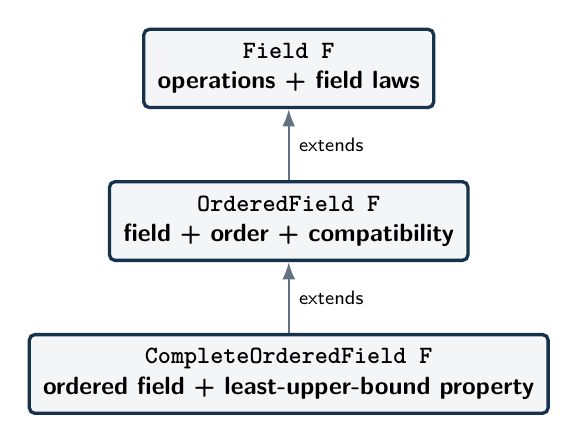
\begin{tikzpicture}[node distance=9mm]
  \node[bundle] (field) {\code{Field F}\\operations + field laws};
  \node[bundle,below=of field] (ordered) {\code{OrderedField F}\\field + order + compatibility};
  \node[bundle,below=of ordered] (complete) {\code{CompleteOrderedField F}\\ordered field + least-upper-bound property};
  \draw[arr] (complete) -- node[right,font=\scriptsize\sffamily]{extends} (ordered);
  \draw[arr] (ordered) -- node[right,font=\scriptsize\sffamily]{extends} (field);
\end{tikzpicture}
\end{center}

\begin{bigidea}
Read \code{[Field F]} as: ``Lean may automatically search for a complete package of
field operations and proofs for the type \code{F}.'' Once found, the parent packages
inside it are also available to instance inference.
\end{bigidea}

The remaining declarations perform four supporting jobs: define useful subtypes,
define predicates for least upper bounds, embed core \code{Nat} values by recursion,
and package a nonnegative distance function.

\section{The outer shell: comments, namespace, and universes}

\subsection{Three kinds of comments}

\begin{lstlisting}
/- ordinary block comment -/
/-! module documentation -/
/-- declaration documentation -/
-- line comment
\end{lstlisting}

Ordinary comments are ignored. A module doc comment beginning \code{/-!} is associated
with the file/module. A declaration doc comment beginning \code{/--} is attached to the
next declaration and can be shown by editor tooling. The roadmap and design prose are
therefore part of the browsable API documentation, not merely visual separators.

\subsection{Namespaces qualify names}

\begin{lstlisting}
namespace aim.analysis
  -- Field is really aim.analysis.Field here.
end aim.analysis
\end{lstlisting}

A namespace prevents short names such as \code{Field} from occupying the global name
space. Inside the namespace, the short name is normally sufficient. Outside, a client
can write \code{aim.analysis.Field}; an \code{open} command could make short names
available without changing their true full names.

\subsection{Universe variables classify types}

\begin{lstlisting}
universe u v
\end{lstlisting}

\code{Type u} is the universe of types at level \code{u}. Universe levels prevent a
``type of all types'' paradox while retaining polymorphism. Most declarations use one
carrier \code{X : Type u}. The distance structure uses two levels because the point
type and value type need not inhabit the same universe:

\begin{lstlisting}
structure Distance (X : Type u) (R : Type v) ...
\end{lstlisting}

Lean computes an appropriate universe for \code{Distance X R}; the author does not have
to force \code{X} and \code{R} into a common level.

\section{Binders: the punctuation that controls elaboration}

Nearly every declaration is a dependent function type. The shape of a binder tells
Lean how callers will supply its argument.

\begin{center}
\begin{tabularx}{\textwidth}{@{}>{\ttfamily}lXl@{}}
\toprule
\normalfont\bfseries Syntax & \bfseries Meaning & \bfseries How supplied \\
\midrule
(X : Type u) & explicit parameter & caller normally writes it \\
\{F : Type u\} & implicit parameter & elaborator infers it from context \\
{[Add X]} & instance-implicit parameter & typeclass search must synthesize it \\
(a b c : F) & several explicit parameters of one type & caller writes values \\
\bottomrule
\end{tabularx}
\end{center}

For example:

\begin{lstlisting}
theorem field_smoke_test {F : Type u} [Field F] (a b c : F) : ...
\end{lstlisting}

\begin{itemize}
  \item \code{F} is inferred from \code{a}, \code{b}, and \code{c}.
  \item the \code{Field F} object is found by instance inference;
  \item the three elements are ordinary explicit arguments.
\end{itemize}

\begin{warningbox}
Square brackets do not mean ``optional.'' They mean ``ask the instance synthesizer.''
Elaboration fails if no appropriate instance can be built, or if search becomes
ambiguous or cyclic.
\end{warningbox}

\section{Data typeclasses and overloaded notation}

Lean notation such as \code{a + b} is not primitive arithmetic. It is syntax whose
meaning depends on a typeclass instance. Conceptually, core classes have fields like:

\begin{lstlisting}
class Add (X : Type u) where
  add : X → X → X

class Zero (X : Type u) where
  zero : X
\end{lstlisting}

Thus \code{[Add X]} supplies a binary operation, and \code{[Zero X]} supplies a chosen
element. The notations are elaborated using the carrier type:

\begin{center}
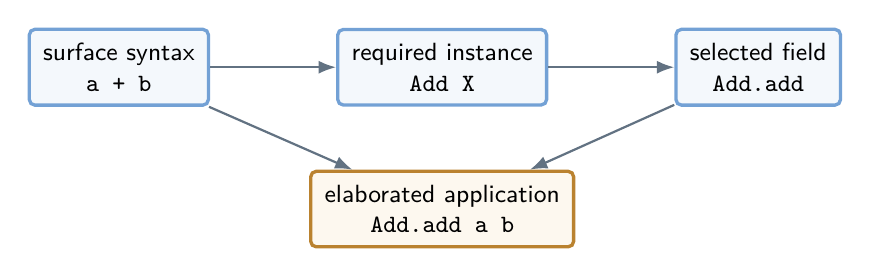
\begin{tikzpicture}[node distance=8mm and 16mm]
  \node[data] (syntax) {surface syntax\\\code{a + b}};
  \node[data,right=of syntax] (need) {required instance\\\code{Add X}};
  \node[data,right=of need] (field) {selected field\\\code{Add.add}};
  \node[generated,below=of need] (term) {elaborated application\\\code{Add.add a b}};
  \draw[arr] (syntax) -- (need);
  \draw[arr] (need) -- (field);
  \draw[arr] (field) -- (term);
  \draw[arr] (syntax) -- (term);
\end{tikzpicture}
\end{center}

The same pattern explains all operation and relation parents in the file:

\begin{longtable}{@{}>{\ttfamily}p{0.18\textwidth}>{\ttfamily}p{0.16\textwidth}p{0.56\textwidth}@{}}
\toprule
\normalfont\bfseries Class & \normalfont\bfseries Notation & \bfseries Data supplied \\
\midrule
\endhead
Zero F & 0 & distinguished zero \\
One F & 1 & distinguished one \\
Add F & a + b & binary addition \\
Mul F & a * b & binary multiplication \\
Neg F & -a & unary negation \\
Inv F & a⁻¹ & unary reciprocal \\
LE F & a ≤ b & non-strict relation \\
LT F & a < b & strict relation \\
Sub F & a - b & binary subtraction \\
Div F & a / b & binary division \\
\bottomrule
\end{longtable}

Numerals are type-directed too. The annotation in \code{(0 : X) ≠ 1} fixes the type of
zero; equality then forces one to have the same type. Elsewhere the surrounding
operation or relation often supplies enough expected type information.

\section{Propositions, proofs, and logical syntax}

In Lean, propositions are types in \code{Prop}; proofs are values of those types. A
class declared \code{: Prop} contains proof data but no computationally relevant
mathematical carrier data.

\begin{lstlisting}
class IsAddAssoc (X : Type u) [Add X] : Prop where
  add_assoc : ∀ a b c : X, a + b + c = a + (b + c)
\end{lstlisting}

This declaration introduces:

\begin{enumerate}
  \item a proposition family \code{IsAddAssoc X}, dependent on a chosen \code{Add X};
  \item a constructor that builds the class from a proof of the field;
  \item a projection \code{IsAddAssoc.add_assoc} that extracts the proof;
  \item typeclass metadata because \code{class}, rather than \code{structure}, was used.
\end{enumerate}

The distinct logical forms appearing across the file are:

\begin{center}
\begin{tabularx}{\textwidth}{@{}>{\ttfamily}lX@{}}
\toprule
\normalfont\bfseries Form & \bfseries Reading \\
\midrule
∀ a : X, P a & for every \code{a}, produce a proof of \code{P a} \\
P → Q & a function taking a proof of \code{P} to a proof of \code{Q} \\
a = b & propositional equality \\
¬ P & abbreviation for \code{P → False} \\
P ∧ Q & a pair containing proofs of both propositions \\
P ∨ Q & a tagged choice containing a proof of one side \\
P ↔ Q & implications in both directions \\
∃ x, P x & a witness \code{x} paired with a proof of \code{P x} \\
\bottomrule
\end{tabularx}
\end{center}

The arrow therefore has two related readings. In \code{X → X → X} it is an ordinary
function arrow. In \code{a ≠ 0 → a * a⁻¹ = 1}, both endpoints are propositions, so the
function consumes one proof and produces another. This is the propositions-as-types
principle in action.

\section{Mixin classes: one reusable pattern}

\subsection{The archetype}

Associativity is the archetypal mixin:

\begin{lstlisting}
class IsAddAssoc (X : Type u) [Add X] : Prop where
  add_assoc : ∀ a b c : X, a + b + c = a + (b + c)
\end{lstlisting}

It says: after a type \code{X} and a particular addition operation have been chosen,
there may be a canonical proof that this operation is associative. The operation is a
dependency, not a field of the mixin. Consequently, two different \code{Add X}
instances would define two different elaborated associativity claims.

\begin{mental}
A data class answers ``what operation do we use?'' A law mixin answers ``what can we
prove about the operation already selected?'' A bundle such as \code{Field F} stores
both answers together and publishes them to instance inference.
\end{mental}

\subsection{The complete mixin catalog}

The other mixins repeat the same declaration mechanism. They need not each be relearned;
only their dependencies and propositions change.

\small
\begin{longtable}{@{}p{0.22\textwidth}p{0.28\textwidth}p{0.43\textwidth}@{}}
\toprule
\bfseries Mixin & \bfseries Required data & \bfseries Law stored \\
\midrule
\endhead
\code{IsAddAssoc X} & \code{Add X} & addition associates \\
\code{IsAddComm X} & \code{Add X} & addition commutes \\
\code{IsMulAssoc X} & \code{Mul X} & multiplication associates \\
\code{IsMulComm X} & \code{Mul X} & multiplication commutes \\
\code{IsZeroNeOne X} & \code{Zero X}, \code{One X} & the identities are distinct \\
\code{IsZeroAdd X} & \code{Zero X}, \code{Add X} & zero is a left additive identity \\
\code{IsAddNeg X} & \code{Zero X}, \code{Add X}, \code{Neg X} & each element plus its negation is zero \\
\code{IsOneMul X} & \code{One X}, \code{Mul X} & one is a left multiplicative identity \\
\code{IsMulInvCancel X} & \code{Zero X}, \code{One X}, \code{Mul X}, \code{Inv X} & nonzero elements cancel with inverses \\
\code{IsMulAdd X} & \code{Add X}, \code{Mul X} & left distributivity \\
\code{IsLERefl X} & \code{LE X} & reflexivity \\
\code{IsLETrans X} & \code{LE X} & transitivity \\
\code{IsLEAntisymm X} & \code{LE X} & antisymmetry \\
\code{IsLETotal X} & \code{LE X} & totality \\
\code{IsLTIffLENotLE X} & \code{LE X}, \code{LT X} & strict order is \(\leq\) plus failure of reverse \(\leq\) \\
\code{IsAddLEAddRight X} & \code{Add X}, \code{LE X} & right translation preserves order \\
\code{IsMulPos X} & \code{Zero X}, \code{Mul X}, \code{LT X} & positive times positive is positive \\
\code{IsOrderComplete F} & \code{LE F} & every inhabited, bounded-above predicate has a least upper bound \\
\code{ArchimedeanProperty F} & \code{OrderedField F} & every value lies below a natural-number cast \\
\bottomrule
\end{longtable}
\normalsize

One-sided laws are deliberate. Commutativity later permits derivation of right identity,
the opposite inverse orientation, and right distributivity. The file stores a compact
axiom basis rather than every convenient theorem.

\section{Instances: rules in a type-directed search program}

An \code{instance} declaration registers a term as a rule available to typeclass
inference. Consider the associativity bridge:

\begin{lstlisting}
instance {X : Type u} [Add X] [IsAddAssoc X] :
    Std.Associative ((· + ·) : X → X → X) :=
  ⟨IsAddAssoc.add_assoc⟩
\end{lstlisting}

Read it from right to left conceptually:

\begin{enumerate}
  \item Goal: build \code{Std.Associative ((· + ·) : X → X → X)}.
  \item Preconditions: synthesize \code{Add X} and \code{IsAddAssoc X}.
  \item Extract the custom proof with \code{IsAddAssoc.add_assoc}.
  \item Put that proof into the one-field standard class using \code{⟨...⟩}.
\end{enumerate}

\subsection{Anonymous functions and operator sections}

\code{((· + ·) : X → X → X)} is a section using centered-dot placeholders. It means
the same function as \code{fun a b : X => a + b}. The type annotation fixes both
placeholder types and prevents ambiguity.

\subsection{Anonymous constructor notation}

Angle brackets tell Lean to use the expected structure or inductive constructor:

\begin{lstlisting}
⟨IsAddAssoc.add_assoc⟩
⟨0⟩
⟨fun a b => a + -b⟩
\end{lstlisting}

The first builds a standard associativity witness, the second builds \code{Nonempty F},
and the third builds \code{Sub F}. The expected result type determines which constructor
the brackets mean.

\subsection{Bridge graph}

\begin{center}
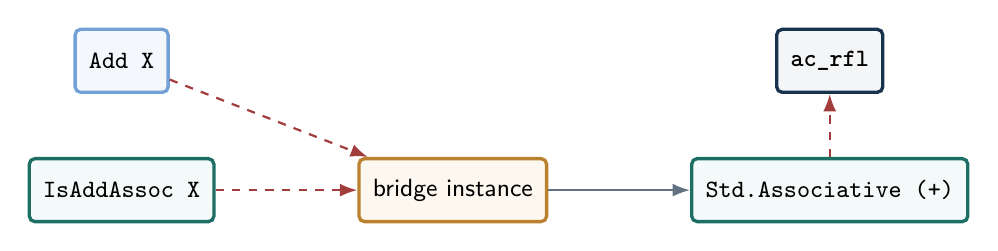
\begin{tikzpicture}[node distance=8mm and 18mm]
  \node[data] (add) {\code{Add X}};
  \node[law,below=of add] (custom) {\code{IsAddAssoc X}};
  \node[generated,right=of custom] (rule) {bridge instance};
  \node[law,right=of rule] (std) {\code{Std.Associative (+)}};
  \node[bundle,above=of std] (tactic) {\code{ac_rfl}};
  \draw[infer] (add) -- (rule);
  \draw[infer] (custom) -- (rule);
  \draw[arr] (rule) -- (std);
  \draw[infer] (std) -- (tactic);
\end{tikzpicture}
\end{center}

Four declarations instantiate this pattern: addition/multiplication crossed with
associativity/commutativity. The bridge avoids coupling the custom educational hierarchy
to a reimplementation of core tactics.

\section{Structure extension and generated parent instances}

\subsection{What \code{extends} means here}

\begin{lstlisting}
class Field (F : Type u)
    extends Zero F, One F, Add F, Mul F, Neg F, Inv F,
      IsZeroNeOne F,
      IsAddAssoc F, IsAddComm F, IsZeroAdd F, IsAddNeg F,
      IsMulAssoc F, IsMulComm F, IsOneMul F, IsMulInvCancel F,
      IsMulAdd F
\end{lstlisting}

\code{Field F} is a class structure whose parents are all the listed classes. An object
of this type contains the data and proof content needed for every parent. Because the
parents are classes, Lean generates projection instances that can recover them.

The ordering matters during elaboration. The data parents occur first. By the time Lean
elaborates \code{IsAddAssoc F}, it can use the inherited \code{Add F}; similarly, the
inverse law can use inherited zero, one, multiplication, and inverse.

\begin{center}
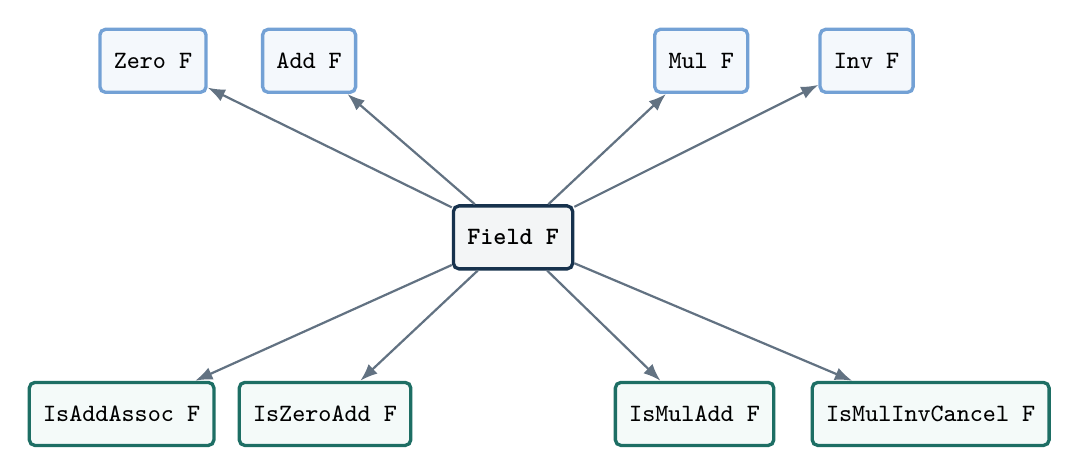
\begin{tikzpicture}[node distance=7mm and 9mm]
  \node[bundle] (field) {\code{Field F}};
  \node[data,above left=14mm and 31mm of field] (z) {\code{Zero F}};
  \node[data,above left=14mm and 12mm of field] (a) {\code{Add F}};
  \node[data,above right=14mm and 10mm of field] (m) {\code{Mul F}};
  \node[data,above right=14mm and 31mm of field] (inv) {\code{Inv F}};
  \node[law,below left=14mm and 30mm of field] (assoc) {\code{IsAddAssoc F}};
  \node[law,below left=14mm and 5mm of field] (zeroadd) {\code{IsZeroAdd F}};
  \node[law,below right=14mm and 5mm of field] (muladd) {\code{IsMulAdd F}};
  \node[law,below right=14mm and 30mm of field] (cancel) {\code{IsMulInvCancel F}};
  \foreach \n in {z,a,m,inv,assoc,zeroadd,muladd,cancel} \draw[arr] (field) -- (\n);
\end{tikzpicture}
\end{center}

The arrows mean ``can project as an instance,'' not logical implication alone. If the
local context contains \code{[Field F]}, a search for \code{[Add F]} or
\code{[IsAddAssoc F]} can follow the generated parent projection.

\subsection{Why no explicit \code{where} block?}

All fields come from parents, so the class body is empty. Lean accepts the declaration
without \code{where}. A concrete field construction will later need to provide values
for the inherited parents, directly or through constructor syntax.

\subsection{The full hierarchy}

\begin{center}
\resizebox{\textwidth}{!}{%
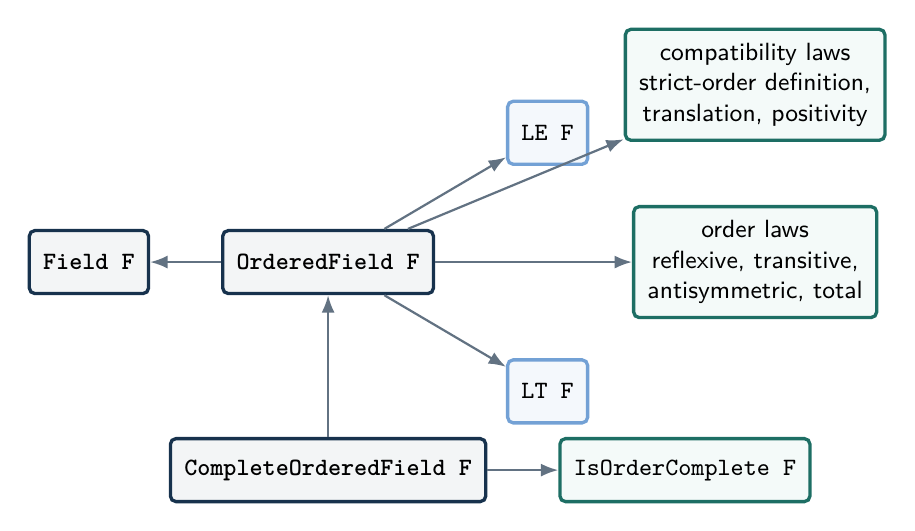
\begin{tikzpicture}[node distance=8mm and 9mm]
  \node[bundle] (of) {\code{OrderedField F}};
  \node[bundle,left=of of] (f) {\code{Field F}};
  \node[data,above right=of of] (le) {\code{LE F}};
  \node[data,below right=of of] (lt) {\code{LT F}};
  \node[law,right=25mm of of] (orderlaws) {order laws\\reflexive, transitive,\\antisymmetric, total};
  \node[law,above=of orderlaws] (compat) {compatibility laws\\strict-order definition,\\translation, positivity};
  \node[bundle,below=18mm of of] (cof) {\code{CompleteOrderedField F}};
  \node[law,right=of cof] (complete) {\code{IsOrderComplete F}};
  \draw[arr] (of) -- (f);
  \draw[arr] (of) -- (le);
  \draw[arr] (of) -- (lt);
  \draw[arr] (of) -- (orderlaws);
  \draw[arr] (of) -- (compat);
  \draw[arr] (cof) -- (of);
  \draw[arr] (cof) -- (complete);
\end{tikzpicture}}
\end{center}

\section{Derived data instances: nonemptiness, subtraction, division}

The field bundle supplies enough primitive data to define additional standard
interfaces.

\begin{lstlisting}
instance {F : Type u} [Field F] : Nonempty F :=
  ⟨0⟩
\end{lstlisting}

Once \code{[Field F]} is present, its generated \code{Zero F} parent makes \code{0 : F}
available. That value witnesses that \code{F} is inhabited. \code{Nonempty F} is a
proposition, so this records existence without choosing computational default behavior.

\begin{lstlisting}
instance {F : Type u} [Field F] : Sub F :=
  ⟨fun a b => a + -b⟩

instance {F : Type u} [Field F] : Div F :=
  ⟨fun a b => a * b⁻¹⟩
\end{lstlisting}

\code{fun a b => ...} is lambda syntax. Subtraction and division are not new primitive
field data in this design; they are computed from addition/negation and
multiplication/inverse.

\begin{center}
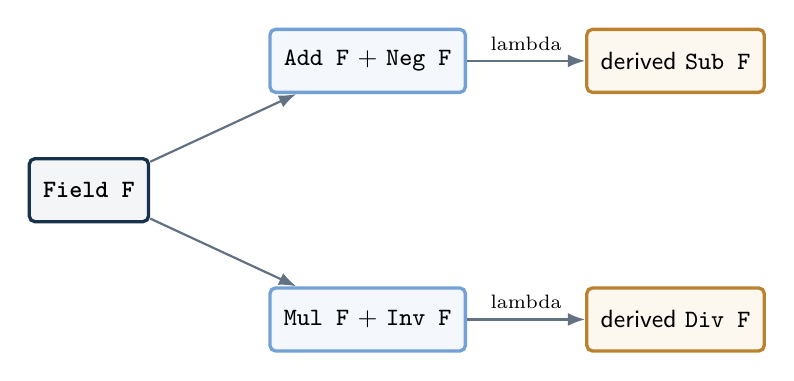
\begin{tikzpicture}[node distance=8mm and 15mm]
  \node[bundle] (field) {\code{Field F}};
  \node[data,above right=of field] (an) {\code{Add F} + \code{Neg F}};
  \node[data,below right=of field] (mi) {\code{Mul F} + \code{Inv F}};
  \node[generated,right=of an] (sub) {derived \code{Sub F}};
  \node[generated,right=of mi] (div) {derived \code{Div F}};
  \draw[arr] (field) -- (an);
  \draw[arr] (field) -- (mi);
  \draw[arr] (an) -- node[above,font=\scriptsize]{lambda} (sub);
  \draw[arr] (mi) -- node[above,font=\scriptsize]{lambda} (div);
\end{tikzpicture}
\end{center}

\subsection{Definitional equality and \code{rfl}}

\begin{lstlisting}
theorem sub_eq_add_neg {F : Type u} [Field F] (a b : F) :
    a - b = a + -b :=
  rfl
\end{lstlisting}

After unfolding the selected \code{Sub F} instance, both sides are literally the same
term. \code{rfl} proves reflexive equality; no algebraic axiom is used. This is
\emph{definitional} or computational equality, stronger than merely having a theorem
relating two independently chosen operations. The division theorem is identical in
syntax category and reasoning.

\section{Predicates as sets and order completeness}

The file represents a set of \code{F}-elements by its membership predicate
\code{s : F → Prop}. Saying \code{s x} means ``\code{x} belongs to the set.'' This avoids
requiring a separate set library.

\begin{lstlisting}
def IsUpperBound {F : Type u} [LE F]
    (s : F → Prop) (a : F) : Prop :=
  ∀ x : F, s x → x ≤ a
\end{lstlisting}

This is a transparent definition: it introduces an abbreviation with computational
content that Lean may unfold. It is not a class and is not searched for automatically.

\begin{lstlisting}
def IsLeastUpperBound ... (s : F → Prop) (a : F) : Prop :=
  IsUpperBound s a ∧
  ∀ b : F, IsUpperBound s b → a ≤ b
\end{lstlisting}

The conjunction packages two proofs: \code{a} is an upper bound, and \code{a} is below
every upper bound.

\begin{center}
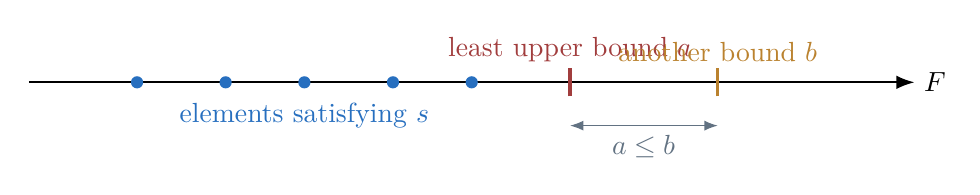
\begin{tikzpicture}[x=1.25cm,y=1cm]
  \draw[-{Latex},thick] (0,0) -- (9,0) node[right]{\(F\)};
  \foreach \x in {1.1,2.0,2.8,3.7,4.5} \fill[blue] (\x,0) circle (2.2pt);
  \node[blue,below=4pt] at (2.8,0) {elements satisfying \(s\)};
  \draw[red!80!black,very thick] (5.5,-0.18) -- (5.5,0.18);
  \node[red!80!black,above=4pt] at (5.5,0) {least upper bound \(a\)};
  \draw[gold!80!black,very thick] (7,-0.18) -- (7,0.18);
  \node[gold!80!black,above=4pt] at (7,0) {another bound \(b\)};
  \draw[{Latex}-{Latex},muted] (5.5,-0.55) -- node[below]{\(a\le b\)} (7,-0.55);
\end{tikzpicture}
\end{center}

\code{IsOrderComplete} turns the least-upper-bound assertion into a reusable class law.
The nested arrows expose its prerequisites:

\begin{enumerate}
  \item choose any predicate \code{s};
  \item supply an existential witness proving it is nonempty;
  \item supply an existential witness proving it has an upper bound;
  \item receive an existentially packaged least upper bound.
\end{enumerate}

\section{Subtypes: values carrying proofs}

\begin{lstlisting}
def RPos (R : Type u) [Zero R] [LT R] : Type u :=
  { x : R // 0 < x }
\end{lstlisting}

The subtype syntax \code{\{ x : R // P x \}} denotes pairs consisting of a value
\code{x : R} and a proof of \code{P x}. For a value \code{p : RPos R}, one can extract
its underlying value and proof conceptually as \code{p.val} and \code{p.property}.

\begin{center}
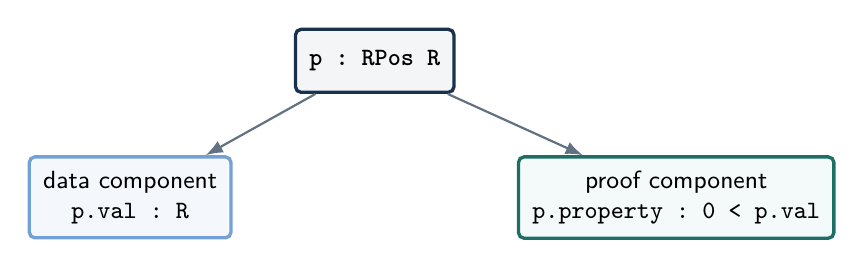
\begin{tikzpicture}[node distance=11mm]
  \node[bundle] (pair) {\code{p : RPos R}};
  \node[data,below left=of pair] (val) {data component\\\code{p.val : R}};
  \node[law,below right=of pair] (proof) {proof component\\\code{p.property : 0 < p.val}};
  \draw[arr] (pair) -- (val);
  \draw[arr] (pair) -- (proof);
\end{tikzpicture}
\end{center}

\code{RNeg} and \code{RNonneg} use exactly the same syntax category with different
predicates. Because each is a \code{def}, it is a named subtype expression rather than
a new opaque primitive type.

\begin{warningbox}
The names begin with \code{R}, but the parameter can be any ordered carrier providing
the requested instances. No real-number construction is required by these definitions.
\end{warningbox}

\section{Recursive construction by pattern matching: \code{natCast}}

\begin{lstlisting}
def natCast {F : Type u} [Zero F] [One F] [Add F] : Nat → F
  | 0 => 0
  | n + 1 => natCast n + 1
\end{lstlisting}

The declaration defines a function from core \code{Nat} to \code{F}. Its equations are
written directly as pattern-matching clauses.

\begin{itemize}
  \item Input pattern \code{0}: return the selected zero of \code{F}.
  \item Successor pattern \code{n + 1}: recursively cast \code{n}, then add the selected
        one of \code{F}.
\end{itemize}

Lean sees that the recursive call is made on the structurally smaller \code{n}, so it
accepts termination automatically. No field laws are needed to define this function;
only the three pieces of operational data used by its equations are required.

\begin{center}
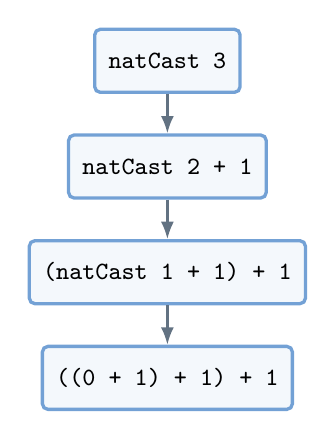
\begin{tikzpicture}[node distance=5mm]
  \node[data] (n3) {\code{natCast 3}};
  \node[data,below=of n3] (n2) {\code{natCast 2 + 1}};
  \node[data,below=of n2] (n1) {\code{(natCast 1 + 1) + 1}};
  \node[data,below=of n1] (n0) {\code{((0 + 1) + 1) + 1}};
  \draw[arr] (n3) -- (n2);
  \draw[arr] (n2) -- (n1);
  \draw[arr] (n1) -- (n0);
\end{tikzpicture}
\end{center}

The result is a repeated-addition embedding candidate. Injectivity and preservation of
addition or multiplication are intentionally future theorems, not consequences of the
definition alone.

\section{A dependent mixin: the Archimedean property}

\begin{lstlisting}
class ArchimedeanProperty (F : Type u) [OrderedField F] : Prop where
  archimedean : ∀ x : F, ∃ n : Nat, x < natCast n
\end{lstlisting}

This mixin depends on the entire ordered-field package rather than listing individual
operations. That package provides \code{LT F} for \code{<} and also, through its
\code{Field F} parent, the zero, one, and addition needed to infer the arguments of
\code{natCast}.

The field says that for each \code{x}, a proof contains both a natural-number witness
\code{n} and evidence of \code{x < natCast n}. The class remains separate even though
the property is intended to be proved later from completeness: separation permits the
same downstream theory to apply to ordered fields whose Archimedean property is given
independently.

\section{Ordinary structures: the revised \code{Distance}}

\begin{lstlisting}
structure Distance (X : Type u) (R : Type v) [Zero R] [LE R] where
  dist : X → X → R
  dist_nonneg : ∀ x y : X, 0 ≤ dist x y
\end{lstlisting}

This is an ordinary structure, not a class. A value \code{d : Distance X R} is passed
explicitly unless some later declaration chooses to install one as an instance. It has
two named fields:

\begin{enumerate}
  \item \code{d.dist x y : R}, ordinary carrier-valued distance data;
  \item \code{d.dist_nonneg x y}, a proof that this value is nonnegative.
\end{enumerate}

\begin{center}
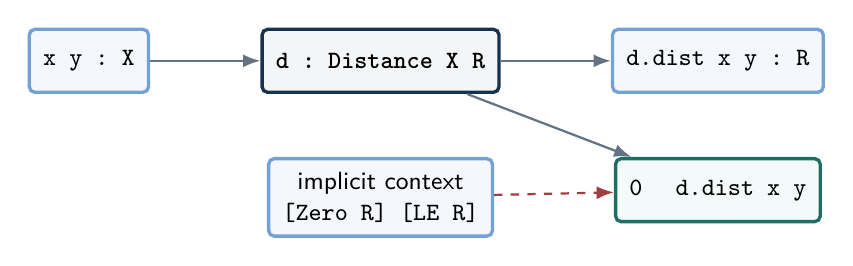
\begin{tikzpicture}[node distance=8mm and 14mm]
  \node[data] (xy) {\code{x y : X}};
  \node[bundle,right=of xy] (d) {\code{d : Distance X R}};
  \node[data,right=of d] (r) {\code{d.dist x y : R}};
  \node[law,below=of r] (p) {\code{0 ≤ d.dist x y}};
  \node[data,below=of d] (inst) {implicit context\\\code{[Zero R] [LE R]}};
  \draw[arr] (xy) -- (d);
  \draw[arr] (d) -- (r);
  \draw[arr] (d) -- (p);
  \draw[infer] (inst) -- (p);
\end{tikzpicture}
\end{center}

Keeping \code{dist} carrier-valued is important: clients can use whatever algebraic
operations \code{R} supports without repeatedly unwrapping a nonnegative subtype. The
proof remains adjacent to the function and is available through a projection. This
structure intentionally states only nonnegativity; symmetry, identity of indiscernibles,
and the triangle inequality would belong to a stronger future metric structure.

\section{Theorem declarations and proof styles}

The smoke tests exercise three distinct proof mechanisms.

\subsection{Direct term proof by projection}

\begin{lstlisting}
theorem field_smoke_test {F : Type u} [Field F] (a b c : F) :
    a + b + c = a + (b + c) :=
  IsAddAssoc.add_assoc a b c
\end{lstlisting}

After the colon comes the theorem's proposition. After \code{:=} comes a term of that
type. The projection has a hidden \code{IsAddAssoc F} instance parameter, which inference
obtains from the \code{Field F} parent.

\subsection{Tactic proof}

\begin{lstlisting}
theorem field_ac_smoke_test ... :
    a + b + c = c + (b + a) := by
  ac_rfl
\end{lstlisting}

\code{by} opens tactic mode. \code{ac_rfl} normalizes expressions modulo associativity
and commutativity. Its required standard witnesses are found through the custom bridge
instances.

\subsection{Definitional proof}

The subtraction and division theorems use \code{rfl}, as discussed earlier. Their
validity comes from unfolding definitions, not from the field-law mixins.

\section{End-to-end inference traces}

\subsection{How \texorpdfstring{\texttt{field\_smoke\_test}}{field_smoke_test} finds associativity}

\begin{tracebox}
\begin{enumerate}
  \item Local context contains \code{instField : Field F}.
  \item The expression \code{a + b} creates a need for \code{Add F}.
  \item Instance search uses the generated \code{Field.toAdd} parent projection.
  \item \code{IsAddAssoc.add_assoc} creates a need for \code{IsAddAssoc F}.
  \item Search uses the generated \code{Field.toIsAddAssoc} projection.
  \item Applying the extracted universally quantified proof to \code{a}, \code{b}, and
        \code{c} produces exactly the target equality.
\end{enumerate}
\end{tracebox}

\subsection{How \texorpdfstring{\texttt{ac\_rfl}}{ac_rfl} crosses the custom/core boundary}

\begin{center}
\resizebox{\textwidth}{!}{%
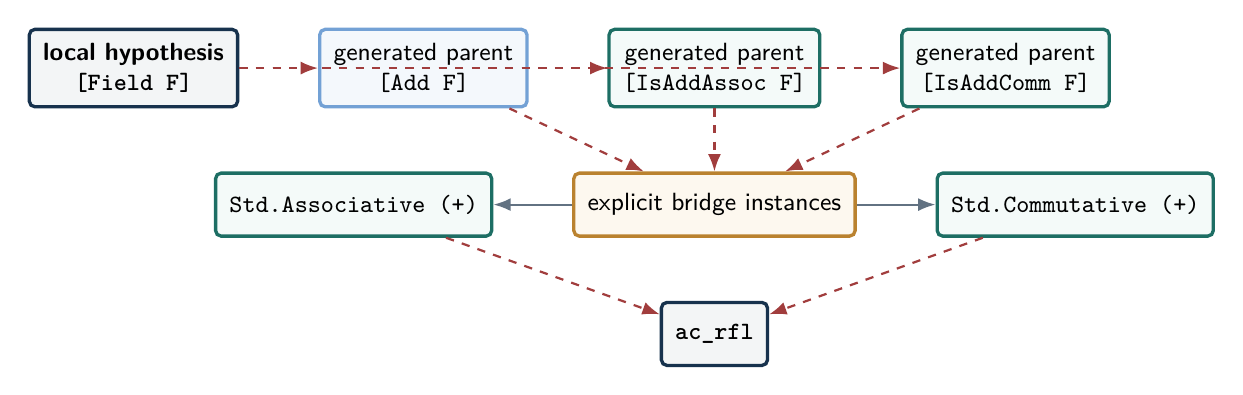
\begin{tikzpicture}[node distance=8mm and 10mm]
  \node[bundle] (context) {local hypothesis\\\code{[Field F]}};
  \node[data,right=of context] (add) {generated parent\\\code{[Add F]}};
  \node[law,right=of add] (assoc) {generated parent\\\code{[IsAddAssoc F]}};
  \node[law,right=of assoc] (comm) {generated parent\\\code{[IsAddComm F]}};
  \node[generated,below=of assoc] (bridges) {explicit bridge instances};
  \node[law,left=of bridges] (stdA) {\code{Std.Associative (+)}};
  \node[law,right=of bridges] (stdC) {\code{Std.Commutative (+)}};
  \node[bundle,below=of bridges] (ac) {\code{ac_rfl}};
  \draw[infer] (context) -- (add);
  \draw[infer] (context) -- (assoc);
  \draw[infer] (context) -- (comm);
  \draw[infer] (add) -- (bridges);
  \draw[infer] (assoc) -- (bridges);
  \draw[infer] (comm) -- (bridges);
  \draw[arr] (bridges) -- (stdA);
  \draw[arr] (bridges) -- (stdC);
  \draw[infer] (stdA) -- (ac);
  \draw[infer] (stdC) -- (ac);
\end{tikzpicture}}
\end{center}

The tactic never needs to know about \code{Field}. It requests standard algebraic
properties of the particular operation. Instance inference connects those requests to
the custom hierarchy.

\subsection{How \code{x < natCast n} elaborates}

\begin{tracebox}
Inside \code{ArchimedeanProperty}, \code{[OrderedField F]} yields \code{LT F} directly
and \code{Field F} transitively. The latter yields \code{Zero F}, \code{One F}, and
\code{Add F}. These solve the implicit parameters of \code{natCast}; its result type is
therefore \code{F}. Both sides of \code{<} now have type \code{F}, so the selected
\code{LT F} relation applies.
\end{tracebox}

\section{Construction: what a future concrete field must provide}

The present file defines interfaces, not a concrete instance. A later construction of a
carrier \code{K} must eventually create a \code{Field K}. Conceptually the process is:

\begin{center}
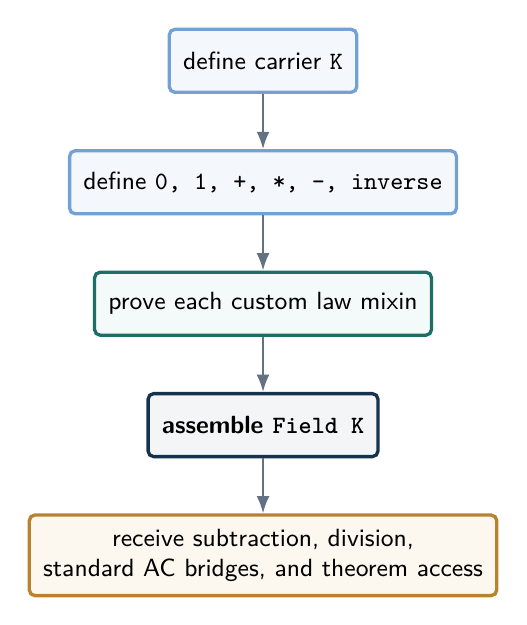
\begin{tikzpicture}[node distance=7mm]
  \node[data] (carrier) {define carrier \code{K}};
  \node[data,below=of carrier] (ops) {define \code{0, 1, +, *, -, inverse}};
  \node[law,below=of ops] (proofs) {prove each custom law mixin};
  \node[bundle,below=of proofs] (bundle) {assemble \code{Field K}};
  \node[generated,below=of bundle] (derived) {receive subtraction, division,\\standard AC bridges, and theorem access};
  \draw[arr] (carrier) -- (ops);
  \draw[arr] (ops) -- (proofs);
  \draw[arr] (proofs) -- (bundle);
  \draw[arr] (bundle) -- (derived);
\end{tikzpicture}
\end{center}

A schematic construction might look like the following; field names generated by
extension can vary, so this is a conceptual template rather than promised copy-and-paste
syntax:

\begin{lstlisting}
instance : Field K where
  -- operation fields or parent instances
  -- proofs for zero_ne_one, add_assoc, ..., mul_add
\end{lstlisting}

Once the instance is registered, declarations with \code{[Field K]} can use it without
receiving an explicit parameter. Local instances can override or specialize behavior,
so a typeclass should represent data intended to be canonical in the relevant scope.

\section{Syntax index for the entire file}

This index groups every distinct syntactic mechanism. Repeated uses differ only in
mathematical content.

\small
\begin{longtable}{@{}p{0.24\textwidth}p{0.29\textwidth}p{0.40\textwidth}@{}}
\toprule
\bfseries Syntax category & \bfseries Representative occurrence & \bfseries Role \\
\midrule
\endhead
module doc comment & \code{/-! ... -/} & file-level generated documentation \\
declaration doc comment & \code{/-- ... -/} & attaches prose to the next declaration \\
namespace & \code{namespace aim.analysis} & qualifies all enclosed names \\
universe variables & \code{universe u v} & polymorphic levels for carrier types \\
explicit binder & \code{(X : Type u)} & caller-provided argument \\
implicit binder & \code{\{F : Type u\}} & inferred ordinary argument \\
instance binder & \code{[Add X]} & argument synthesized by typeclass search \\
class in \code{Prop} & \code{class IsAddAssoc ... : Prop} & searchable law package/mixin \\
class with parents & \code{class Field ... extends ...} & searchable combined data/law bundle \\
ordinary structure & \code{structure Distance ...} & explicit record with data and proof fields \\
definition & \code{def IsUpperBound ... :=} & transparent named term/type \\
recursive definition & \code{def natCast ... | ...} & terminating function by pattern matching \\
instance declaration & \code{instance ... : Sub F :=} & rule registered for typeclass inference \\
theorem declaration & \code{theorem ... : P := proof} & named proof term \\
universal quantifier & \code{∀ x : F, ...} & dependent function over every value \\
existential quantifier & \code{∃ x : F, ...} & witness paired with proof \\
logical connectives & \code{→ ∧ ∨ ↔ ¬} & functions and proof-combining types \\
operator notation & \code{+ * - / ≤ < ⁻¹} & syntax resolved through data instances \\
operator section & \code{(· + ·)} & anonymous binary function \\
lambda & \code{fun a b => ...} & explicit anonymous function \\
anonymous constructor & \code{⟨...⟩} & constructor inferred from expected type \\
subtype & \code{\{x : R // P x\}} & carrier value bundled with a proof \\
pattern clause & \code{| n + 1 => ...} & branch of a recursive definition \\
term proof & \code{IsAddAssoc.add_assoc a b c} & direct proof expression \\
tactic proof & \code{by ac_rfl} & tactic generates a proof term \\
reflexivity proof & \code{rfl} & closes definitional equality \\
type annotation & \code{(0 : X)} & fixes an otherwise ambiguous expected type \\
qualified name & \code{Std.Associative} & references declaration from another namespace \\
\bottomrule
\end{longtable}
\normalsize

\section{A disciplined way to read similar Lean files}

When encountering a declaration in this library, use the following visual checklist:

\begin{enumerate}
  \item \textbf{Find the result sort.} Is it a \code{Type}, a \code{Prop}, a theorem, or
        an instance?
  \item \textbf{Classify every binder.} Parentheses, braces, and brackets imply different
        elaboration behavior.
  \item \textbf{Inventory notation dependencies.} Every overloaded symbol requires a
        data instance.
  \item \textbf{Separate data from laws.} Ask which declarations choose operations and
        which merely prove properties.
  \item \textbf{Follow \code{extends} arrows.} These often explain where a missing
        instance comes from.
  \item \textbf{Follow bridge instances.} A tactic may request a standard interface even
        when the local hierarchy uses custom names.
  \item \textbf{Distinguish computation from theorem proving.} \code{rfl} reflects
        definitional reduction; a projection extracts an assumed law; a tactic constructs
        a new proof using available laws.
\end{enumerate}

\begin{bigidea}
The central wiring pattern of this file is:
\[
\begin{aligned}
\text{carrier} &\longrightarrow \text{operation instances}
  \longrightarrow \text{law mixins} \\
&\longrightarrow \text{bundled hierarchy}
  \longrightarrow \text{generated parent instances} \\
&\longrightarrow \text{theorems/tactics}.
\end{aligned}
\]
Once this chain is visible, most punctuation in the file stops looking ceremonial: each
piece tells the elaborator where an input comes from and tells instance inference which
edges it may traverse.
\end{bigidea}

\section{Compact glossary}

\begin{description}[style=nextline,leftmargin=0pt]
\item[Carrier] The underlying type whose elements are being studied, such as \code{F}.
\item[Elaboration] Lean's conversion of convenient surface syntax into a fully typed term
with implicit arguments and instances filled in.
\item[Instance inference] Type-directed search for values whose parameters use square
brackets.
\item[Mixin] A small reusable class, usually proposition-valued here, expressing one law.
\item[Parent projection] A generated function/instance extracting an extended class from
a larger class.
\item[Definitional equality] Equality visible by computation/unfolding, provable by
\code{rfl}.
\item[Propositional equality] The equality type \code{a = b}; it may require an actual
proof using laws.
\item[Subtype] A value of a carrier paired with proof that it satisfies a predicate.
\item[Predicate-as-set] A function \code{F → Prop}; membership is function application.
\item[Canonical data] Data intended to be found automatically as a typeclass instance.
\end{description}

\vfill
\begin{center}
\color{muted}\sffamily
Prepared as a code-specific learning companion for the mathlib-free
\textit{Adventures in Mathematics} project.
\end{center}

\end{document}
